\chapter{Implementing a Linux KVM TCB in Rust}
\label{sec:rewrite}

%We want to rewrite SeKVM in Rust.
%We first forward port SeKVM from 4.18 to 5.15, this is to use newer features
%e.g. LTO.
%Then we employ the two pass method.

%\todo{TODO: The first sentence does not make sense, one cannot enhance the
%security of SeKVM, it is formally verified. Also mention \rustsec{} has the
%same design as SeKVM.}
The goal of this work is to leverage Rust's safety features in a hypervisor TCB.
Our Rust-based hypervisor, \rustsec{}, follows the design described in
\autoref{sec:sekvmintro}, and is based upon the SeKVM implementation.
%We experimented with its reduced TCB that is designed with security in mind.
We first forward ported SeKVM from its original
Linux 4.18 version to the newest long term support version Linux 5.15 at the
time of development.
By forward porting we benefit from Linux's advancements including performance
optimizations such as Link-Time-Optimization (LTO) and energy aware scheduling.
And new kernel security features including \code{clang} shadow call stacks,
branch target identification, control flow integrity (CFI), ARM Memory Tagging
Extension (MTE), ARM pointer authentication, and randomized stack offset per
system call.

%to take advantage of various new kernel features, for
%example  for better performance, ARM Pointer Authentication (5.0), Energy Aware Scheduling (5.0)
%clang shadow call stack, branch target identification (5.8), MTE (5.10), clang CFI (5.13), randomized stack offset per syscall (5.13)

Once the forward port of SeKVM to Linux 5.15 is done, we then rewrote
the KVM TCB in Rust.
This chapter describes the challenges that arose when implementing a
Rust-based KVM TCB, and the techniques we employed to solve them.

\section{Integrating Rust and Linux}

%challenge: Linux 5.15 does not include Rust support
%
%solution: our way of source code organization, build system integration,
%how we link Rust and C, data layout issues, etc.

Linux 5.15, which is the latest long term support kernel version at the time of
\rustsec{} development, does not support Rust as a development language.
Therefore, we had to integrate Rust code with the rest of the Linux kernel.
We implement \rustcore{} in a single crate on the \code{no\_std} environment
and compile it into a single static library \code{libkrustvm.a}.
The static library is then linked
with the rest of the kernel to create the final kernel image.
We created a new subdirectory in Linux's source path \code{arch/arm64/krustvm}.
Within it contains the \rustcore{} crate and the \code{Makefile} for this
directory. To integrate building \code{libkrustvm.a} and linking it with the
rest of the kernel, we add following to the Makefile:
\begin{enumerate}
\item{append \code{libkrustvm.a} to Kbuild built-in object goals \code{obj-y} by adding the line \code{obj-y += libsekvmrs.a}}
\item{define Makefile target
\begin{listing}[hbtp]
    \begin{minted}{Makefile}
$(obj)/libkrustvm.a: $(src)/krustvm/src/*.rs
        cargo build --release --target=aarch64-unknown-linux-gnu
    \end{minted}
    \label{lst:Makefile}
    \vspace{-1.2cm}
\end{listing}
to instruct \code{make} to use \code{cargo} to generate \code{libkrustvm.a}.
}
\item{link \code{libkrustvm.a} to generate object file \code{krustvm.o}}
\end{enumerate}
The Makefile in \code{arch/arm64/krustvm} generates \code{krustvm.o},
and the kernel build system will then link this file with all other object
files in the kernel and produce the final kernel image.

KVM separates EL2 code from EL1 by grouping EL2 code in a section
\code{.hyp.text}, then mapping that section in EL2's address space at
initialization.
In \rustcore{}, attribute \code{\#[link\_section = ".hyp.text"]} is prepended
to all code that should be run in EL2, so that they get placed in the
\code{.hyp.text} section as well.
Our implementation is compatible with the Linux kernel codebase. For example, we
ensure the page size definition is identical in \rustcore{} and KVM.
Also, we share types like \code{kvm\_vcpu} between Linux and \rustcore{}.
These type definitions are generated automatically
with the tool \code{bindgen}~\cite{bindgen}.
For constants that are used by both Linux and \rustcore{},
we copy them from C to Rust manually.
Due to the limited support of macro in \code{bindgen}
and the heavy usage of Linux,
we do not use it to generate constants.
Regarding alignment, field layout order, and padding of custom types,
we use the Rust attribute \code{\#[repr\-(C)]}
that ensures the data layout of the marked type has the same layout as in C.

Whenever an exception gets taken to EL2, the CPU switches its exception level
to EL2, saves the program status and exception syndrome, and jumps to the
preassigned exception vector.
We modify the exception vectors, which are written in assembly, to call
\rustcore{}'s entry point functions instead of the original C handlers to
transfer the control flow to our Rust code.
%Rust functions in \rustcore{} are invoked in exception vectors.
%This is the place where our Rust code in \rustcore{} comes into play.
%The exception vectors are implemented in assembly, they call Rust
%exception handlers after it switches the register context to EL2.

\section{Bringing up \rustsec{} on Real Hardware}

We chose the Raspberry Pi model 4B (Rpi-4B) to verify our implementation on
real hardware.
%This section describes the problem that occured when trying to run SeKVM on
%Rpi-4B, and how we solved the issue.
SeKVM's trusted core \secore{} originally reserved its private memory by
defining global symbols whose addresses reside right after the kernel image,
in the Linux kernel linker script.
\secore{} then references those symbols to access and utilize the reserved
memory.
However, there exists an unusable hole in Rpi-4B's physical memory address
space, and the bootloader of Rpi-4B places the kernel image before the hole,
resulting in an overlap of \secore{}'s private memory and the unusable hole
(\autoref{fig:overlap}). This makes SeKVM unable to initialize on Rpi-4B.

\begin{figure}[hbtp]
    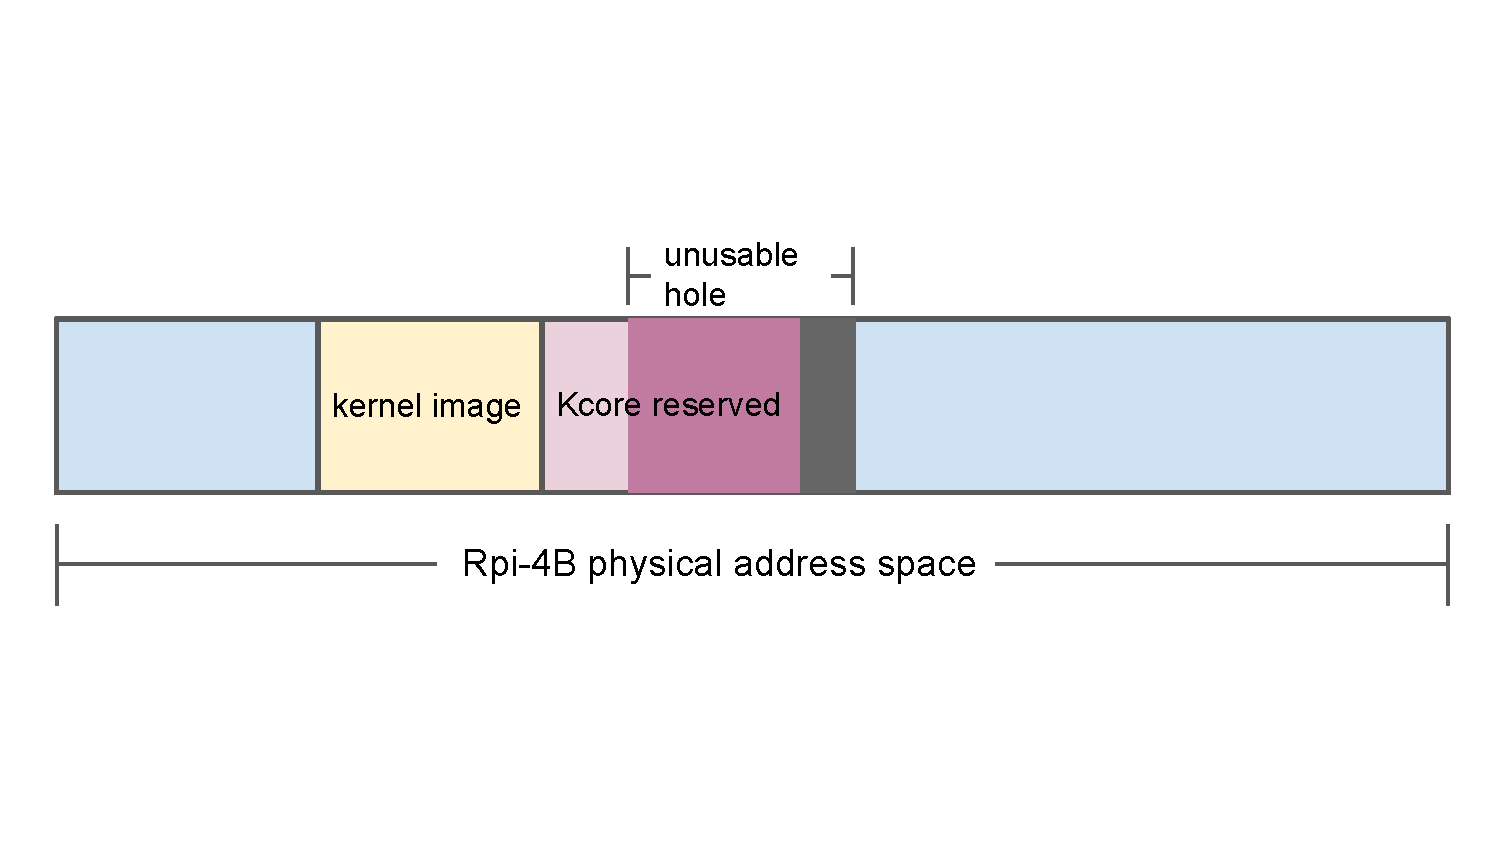
\includegraphics[scale=0.60]{figures/overlap.pdf}
    \caption{Kcore overlaps the unusable hole on Rpi-4B}
    \label{fig:overlap}
\end{figure}

To solve this issue for \rustsec{}, instead of allocating memory in the linker
script, we first locate a range of memory which does not overlap with the
unusable hole of Rpi-4B and the kernel image, then add a new memblock that to
correspond to the \rustcore{}'s private memory. We mark it as reserved by
calling \code{memblock\_reserve}, so that the kernel does not accidentally
access this memory range (\autoref{fig:rcorereserved}).
The global symbols previously defined the Linux kernel linker script have also
been changed to macros that expand into addresses in the reserved range for
\rustsec{}'s \rustcore{} usage.

\begin{figure}[H]
    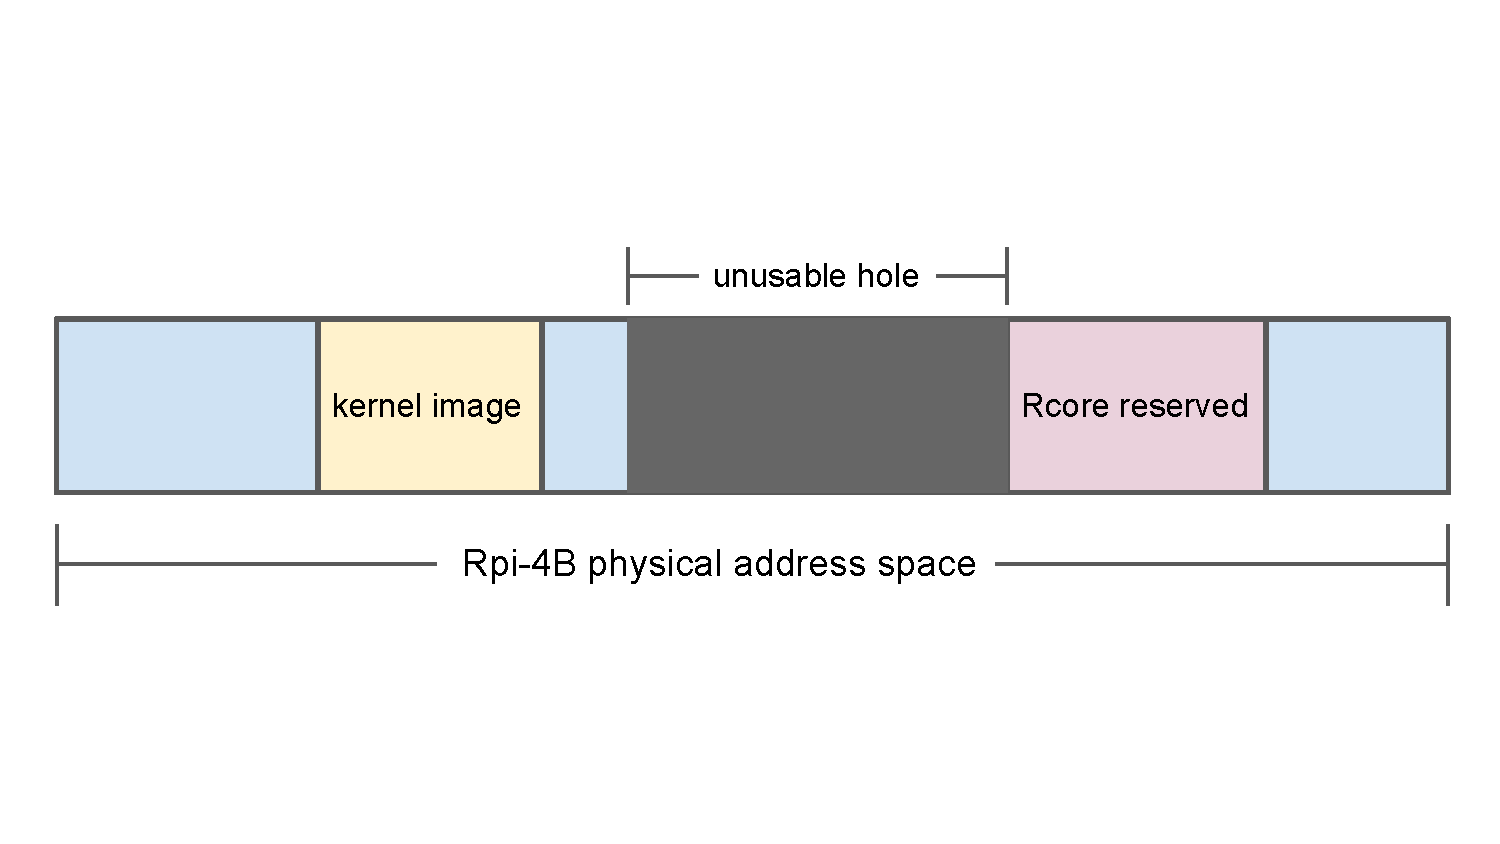
\includegraphics[scale=0.60]{figures/rcore_reserved.pdf}
    \caption{Overlap prevention}
    \label{fig:rcorereserved}
\end{figure}

\section{Rewriting C-based \secore{} into Rust-based \rustcore{}}

%challenge: difficult to do a top-down design due to the difficulty to debug
%and complexity of a hypervisor (is this challenge kinda weak?)
%
%solution: two pass method, first function-by-function rewrite, then remove
%unsafe and redesign after we have a working Rust hypervisor, and leverage
%Rust to achieve a stronger memory region isolation guarantee.

Given the high complexity of the KVM hypervisor and \secore{},
it is clear from the beginning that
a top-down approach to a Rust rewrite would be error-prone and difficult to test.
Therefore, we elected to start the rewriting effort bottom-up,
where all previous C functions in the TCB are rewritten in Rust, one by one.
This incremental approach allows us to test one rewritten function at a time,
reducing the risk of introducing bugs.
%One major downside of this approach is that it is difficult to rewrite a single
%function in a Rust-idiomatic and safe way.
One major downside of this approach is the difficulty of rewriting individual
functions in a manner that adheres to Rust's idiomatic practices.
Furthermore, it may result in a lot of \code{unsafe} blocks.
We solve these issues by adding a second phase to the Rust rewrite;
after the initial function by function rewrite, we removed unnecessary
\code{unsafe} blocks, refactored the code to be more Rust-idiomatic,
and leveraged Rust features to enhance \rustcore{} memory safety.
We discuss the features used to secure \rustcore{} memory accesses in
\autoref{sec:securercore}.

\subsection{Rust Code Organization}
pub

\subsection{Unsafe Rust Usages}

A small part of \rustcore{}'s implementation is coded in unsafe Rust.
The source of unsafe Rust includes inline assembly, the Foreign Function
Interface (FFI), KVM ARM Per-CPU variables, and raw pointer accesses.
The first three categories are discussed in this section,
and for raw pointer usages, \autoref{sec:securercore} shows how we check for
each raw pointer usage scenario and guarantee their memory safety.

\textbf{Inline Assembly.}
Inline assembly are used for system instructions and system register accesses.
For example, TLB invalidation instructions must run when \rustcore{} updates the
NPTs, and the \code{VTTBR\_EL2} register must be switched when preparing to run
a guest VM.
We make use of Rust's built-in module \code{core::arch::asm} to insert inline
assembly. For system register accesses, the \code{aarch64-cpu} crate
\cite{aarch64cpu} is imported into our \rustcore{} crate, it provides a clean
API for reading and writing AArch64 system registers. The inline assembly used
for the actual register accesses are abstracted behind safe APIs.

\textbf{FFI.}
FFIs are used for calling longer assembly routines, such as the cache
invalidation routine, and \code{\_\_guest\_enter} for context switching general
purpose registers and entering guest VMs.

\textbf{KVM ARM Per-CPU Variables in Rust.}
Using KVM ARM Per-CPU variables is special case for unsafe Rust.
Mainline KVM has its EL2 per CPU variable mechanism; it is implemented by first
allocating enough space for all cores to have a copy of the per CPU variables,
then, for each core, it records the offset from its copy of the variables to the
base copy. This per-core offset is then stored in each core's \code{TPIDR\_EL2}
system register. When the need to access a per CPU variable arrives, the
base address is first acquired by referencing a global variable, then adding
\code{TPIDR\_EL2}'s value to the variable's address. \rustsec{} continues to use
this mechanism by declaring the symbol which corresponds to the base address as
a Rust extern static variable, take its raw address, then add the value in
\code{TPIDR\_EL2} to it. This approach requires three \code{unsafe} statements,
first from reading the address of the extern static variable, then reading
\code{TPIDR\_EL2} via inline assembly, and lastly, another \code{unsafe} to
dereference the calculated address. Concurrent accesses will not pose a problem
since each core accesses a different address.

